\chapter{Related Work}
\label{cha:Related Work}
\acresetall


The development of self-driving cars represents one of the most intricate and ambitious challenges in the field of engineering, robotics and \ac{AI}. The complexity and variability of real-world driving environments make this task extremely difficult. The environments include unpredictable actors, such as other drivers, pedestrians, and animals, as well as changing weather and road conditions. The environments include uncounted edge cases that are difficult to anticipate and code for explicitly. Consequently, many researchers and institutions include advanced \ac{ML} techniques in their approaches towards solving autonomous driving.

The development of autonomous driving systems started with driver assistance systems in the 1970s. These systems focus on assisting the driver in specific tasks, such as lane keeping, adaptive cruise control, and parking. This reduces the problem complexity. However modern self-driving systems aim to achieve full autonomy. For example the Tesla autopilot is capable of driving in many environments without human intervention.

This thesis will use \acl{RL} in the training of an autonomous driving agent. The agent is equiped with a single camera sensor. The agent's behaviour is controlled by a \ac{CNN} policy that processes the visual input. The policy has to learn a specific self driving task with reduced complexity. The self-driving task is identical to previous research at the ScaDS.AI by \textcite{maximilian}. However the agent's design and training is very different.
The task consists of a simplified environment. The environment consists of an enclosed arena with different tracks that the agent has to complete. The tracks consist of a series of goals that the agent has to drive through. The tracks are grouped in three difficulty levels \ref{fig:track_examples}.
The environment is simulated with three light settings, bright, standard and dark \ref{fig:light_setting_examples}. The trained agent has to learn to navigate at all difficulty levels and light settings.

\begin{figure}
    \centering
    \subfigure[Easy]{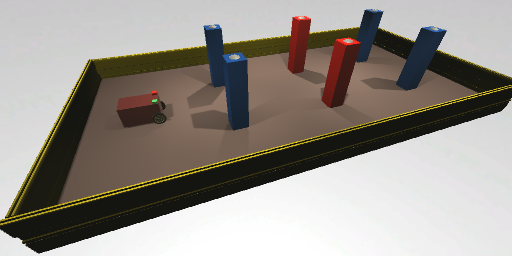
\includegraphics[width=0.3\textwidth]{Bilder/image_printer_images/evaluation_easy.png}}\qquad
    \subfigure[Medium]{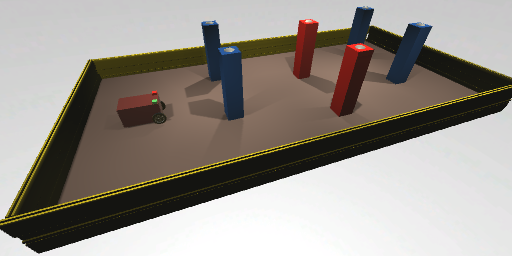
\includegraphics[width=0.3\textwidth]{Bilder/image_printer_images/evaluation_medium.png}}\qquad
    \subfigure[Hard]{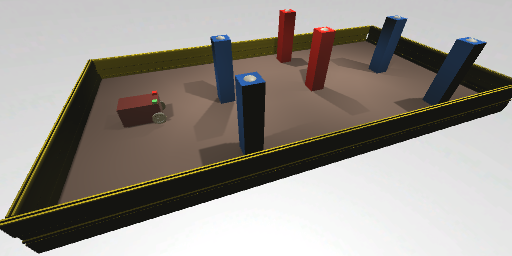
\includegraphics[width=0.3\textwidth]{Bilder/image_printer_images/evaluation_hard.png}}\\
    \caption{Example tracks for each difficulty level}
    \label{fig:track_examples}
\end{figure}

\begin{figure}
    \centering
    \subfigure[Agent Camera Bright]{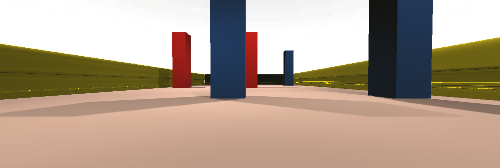
\includegraphics[width=0.3\textwidth]{Bilder/image_printer_images/light_setting_bright_pov_no_preprocessing.png}}\qquad
    \subfigure[Agent Camera Standard]{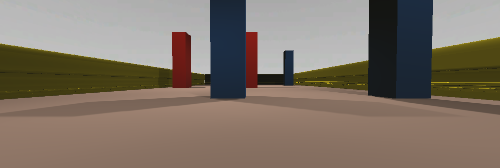
\includegraphics[width=0.3\textwidth]{Bilder/image_printer_images/light_setting_standard_pov_no_preprocessing.png}}\qquad
    \subfigure[Agent Camera Dark]{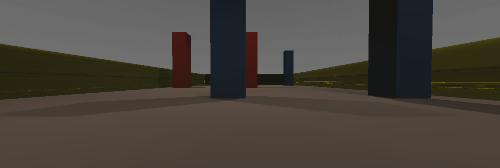
\includegraphics[width=0.3\textwidth]{Bilder/image_printer_images/light_setting_dark_pov_no_preprocessing.png}}\\
    \subfigure[Arena Bright]{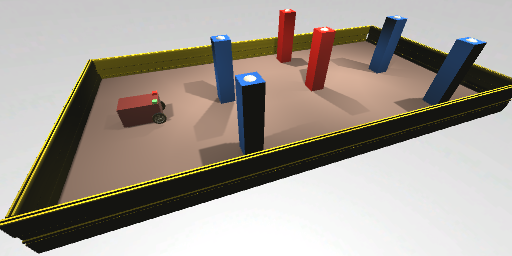
\includegraphics[width=0.3\textwidth]{Bilder/image_printer_images/light_setting_bright_arena.png}}\qquad
    \subfigure[Arena Standard]{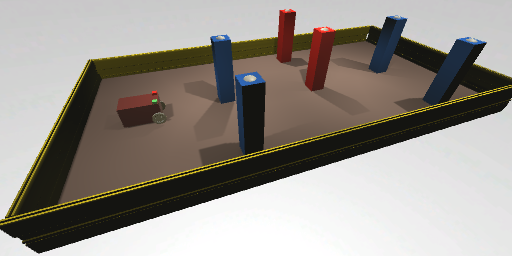
\includegraphics[width=0.3\textwidth]{Bilder/image_printer_images/light_setting_standard_arena.png}}\qquad
    \subfigure[Arena Dark]{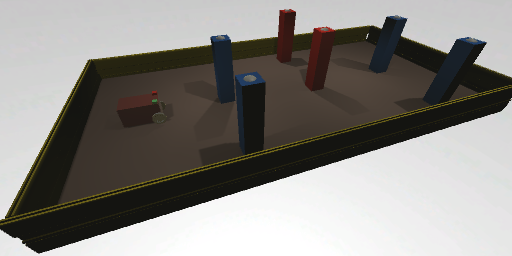
\includegraphics[width=0.3\textwidth]{Bilder/image_printer_images/light_setting_dark_arena.png}}\\
    \caption{Light settings}
    \label{fig:light_setting_examples}
\end{figure}

Research relating to \ac{RL} algorithms, \acp{CNN} and self-driving will be reviewed. The review will highlight the key ideas and approaches that will be used in this thesis to build an autonomous driving agent resistant towards light changes.


\section{Self-Driving}

\acp{NN} have been used in the domain of self driving for a long time. \textcite{alvinn} developed one for the first self driving systems with \acp{NN} in 1989. The system was developed for road following. The system used a camera image and a laser range finder as input. Compared to current network architectures, they used a very small fully connected \ac{NN}. The network was trained using synthetic data. The data consisted of generated road images and steering commands. The network was trained using backpropagation to reproduce the steering commands. This approach did not use \ac{RL}. The system was able to follow roads in real-life under certain conditions.
\textcite{alvinn} highlighted the advantages of \acp{NN} for self-driving. The training data, not the programmer, determines the salient image features. This has proven to be true with the recent success of \acp{CNN} in the domain of self-driving \textcite{drl_for_ad}.


There has been a lot of progress in the domain of self-driving in recent years. Sophisticated self-driving algorithms consist of many hardware and software components to achieve satisfying performance. Hardware components include various imaging approches such as Radar, Lidar and cameras \autocite{drl_for_ad}. Termometers and other hardware components are also used, for example to determine weather conditions. 
Software components might include separate object detection, occupancy and planning. For example Tesla's self-driving builds these components on top of a shared backbone that uses \acp{CNN} \autocite{howteslaautopilot}.
% (CNN is ResNet)

Self-driving in a real world environment is a very complex task, especially when including other traffic participants. Modern self driving agents consist of multiple complex components that interact with each other \autocite{drl_for_ad}. Multiple interacting components are shown in figure \ref{fig:ad_components}. The Scene Understanding components build a model of the current surroundings. The Decision making \& Planning components use this model to decide and execute the next actions.
The components are implemented using different algorithms and \acp{NN}. This can require seperate data collection, training and evaluation processes for the components. An example is the path prediction by Tesla \textcite{tesla_youtube} in 2019. This component is trained using \ac{IL} on a large dataset of human driving behaviour.

\begin{figure}
    \centering
    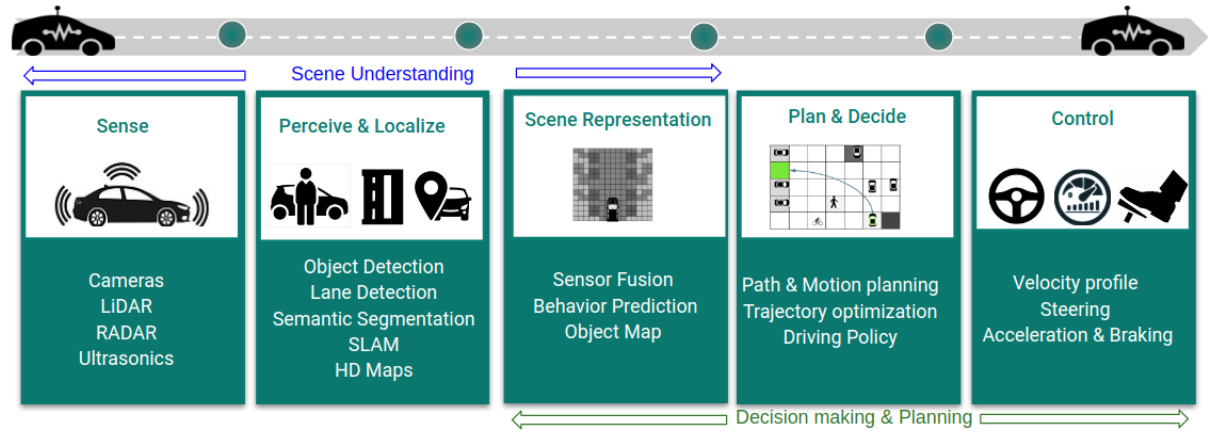
\includegraphics[width=0.8\textwidth]{Bilder/ad_components_from_paper_drl_for_ad.png}
    \caption{Components in a modern autonomous driving system's pipeline. Image from \textcite{drl_for_ad}}
    \label{fig:ad_components}
\end{figure}

An autonomous driving system with similarly complex components is not feasible for this thesis. The simplified nature of the task and previous work by \textcite{maximilian} suggests this is not required.
% The agent in this thesis uses a single \ac{CNN} to process the visual input and make decisions instead. I aim to contribute to the domain by expanding on previous research and focus on the training of a \ac{CNN} agent. 


\subsection{Previous Work at ScaDS.AI}
This thesis builds directly upon the work of \textcite{jonas_koenig}, \textcite{merlin_flach} and \textcite{maximilian}. 
\textcite{jonas_koenig} built a self-driving agent that was trained to avoid collisions in a simulated arena. The agent used a hand-crafted preprocessing pipeline to extract features from visual input. The features represent the obstacles that the agent has to avoid. The agent's behaviour was controlled by a policy that consisted of a \ac{NN}. This network used the extracted features as inputs. It was trained using an evolutionary approach in simulation .

\textcite{merlin_flach} investigated the feasibility of transferring this agent to the real world. The research showcased many challenges. The challenges are caused by differences between the simulated and real-life environments, the Simulation-To-Reality gap. The most notable problem was the object recognition part. The preprocessing pipeline had difficulties recognizing the objects in the real world. This results in further problems for the agent, since the agent's policy is based on the extracted features.

\textcite{maximilian} investigated a different task than the two previous papers. An agent was trained to traverse a track by driving through a sequence of goals. The same tracks are used in this paper. The agent used a preprocessing pipeline to extract object features similar to \textcite{jonas_koenig}. The \ac{NN} policy was trained using the \ac{PPO} \ac{RL} algorithm developed by \textcite{ppo}. The agent could traverse the tracks, its performance decreased for tracks of higher difficulty. Further evaluation of the agent under different light settings showed that the agent is not robust against changing light conditions. The preprocessing pipeline was not able to extract the necessary features reliably under different light settings. This resulted in a performance collapse.

The instability of the hand-crafted preprocessing pipeline and promising results by \acp{CNN} from other RL researchers in the domain of self-driving \textcite{neptune} motivate the choice of \acp{CNN} as the feature extraction method in this thesis. 


\section{\acl{RL}}

% data not programmer decides the salient image pixels (bedeutungsvollen)
\subsection{Introduction to \ac{RL}}

\ac{RL} algorithms have been around for a long time, but only recently have they been able to achieve superhuman performance in games and control tasks \autocite{atari}. \ac{RL} algorithms formalize the problem as consisting of an environment and a policy $\pi$. The environment consists of a state space, an action space and a reward function that takes state-action pairs as input. Reward functions assign positive rewards to actions that are deemed to be desirable by the environment designers, for example scoring a goal in a football match. Reward function can also assign negative rewards to undesirable actions, for example collisions in a driving simulation. 

The goal of \ac{RL} algorithms is to build an agent that interacts with its environment and maximizes the cumulative reward over time. The policy selects actions given an observation. It controls the agents behaviour \autocite{rlbook2020}. It is trained by the \ac{RL} algorithm to learn the desired behaviour. The trained policy can then be used to solve problems in the environment. 

The agent interacts with the environment during the training phase of RL algorithms. The policy takes some representation of the environment's state as input and selects actions to execute in the environment. The selected actions are executed in the environment by the agent which results in a new state. The reward function assigns rewards to these state transitions.
The observed rewards are then used to update the policy \ref{fig:rlcycle}.

\begin{figure}
    \centering
    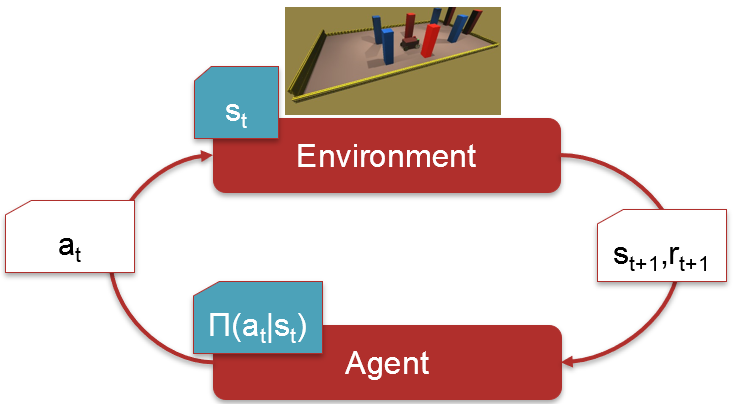
\includegraphics[width=0.4\textwidth]{Bilder/rl_cycle.png}
    \caption{RL Training Cycle: The agent selects action $a_t$ based on policy $\pi(a_t|s_t)$ at state $s_t$ and receives the next state $s_{t+1}$ and rewards $r_{t+1}$ from the environment. The states, actions and observed rewards are used to update the policy.}
    \label{fig:rlcycle}
\end{figure}

\subsection{Classification of \ac{RL} Algorithms}

\ac{RL} algorithms are classified into two major groups. RL algorithms that use a model of the environment are called model-based algorithms, algorithms without such models are called model-free algorithms. Algorithms from both groups have been successfully used in a wide range of applications, model-based algorithms are often much more complex but have been shown to be successful at many tasks that require planning \autocite{alphagoimprovementmuzero}. Model-free approaches are often simpler and more flexible. They have shown great success in various control tasks by \textcite{atari}.

\begin{figure}
    \centering
    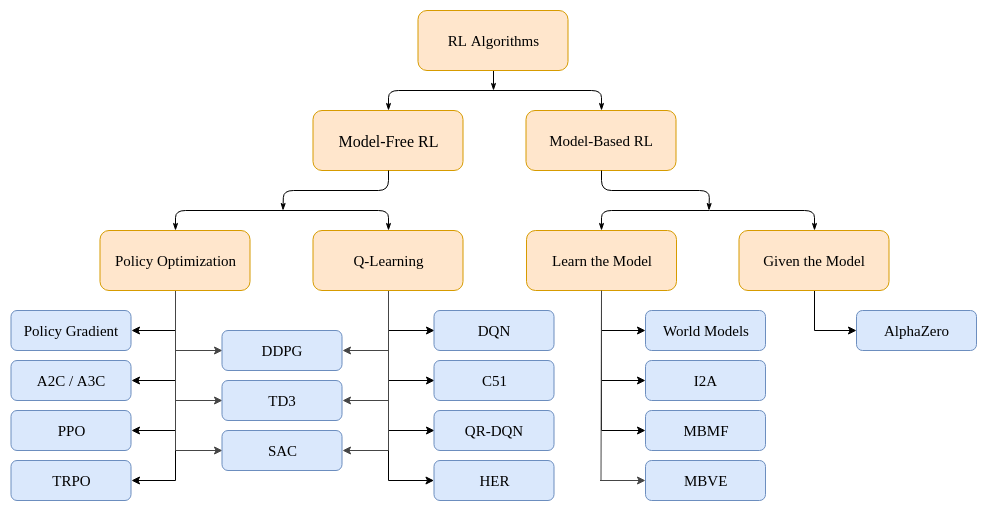
\includegraphics[width=0.8\textwidth]{Bilder/openai_spinningup_taxonomy.png}
    \caption{Taxonomy of \ac{RL} algorithms from OpenAI's Spinning Up course \autocite{spinningup}}
\end{figure}

\subsubsection{Model-Free \ac{RL} Algorithms}

Model-free \ac{RL} algorithms take actions in an environment without an internal representation of the environment. Model-free algorithms learn from direct interactions with the environment.

\paragraph{Value-based algorithms}
Model free algorithms can be further divided into two families. The first family are value-based approaches. These algorithms learn a function that assigns state-action pairs a value. This function is called the value function. This value represents the expected future reward Q.
 
The policy is not trained directly. The policy selects actions based on this value function instead. The state-action pair with the highest Q-value is selected for a given state.

The training process of the value function is done by updating the Q-values based on the observed rewards. The Q-learning algorithm is an early and common example of value-based algorithms \textcite{rlbook2020}. The Q-learning algorithm updates the values based on the observed rewards and the maximum Q-value of the next state: \[Q(S_t, A_t) = Q(S_t, A_t) + \alpha (R_{t+1} + \gamma \max_a Q(S_{t+1}, a) - Q(S_t, A_t))\]
$\alpha$ is the learning rate. It determines how quick values are changed. $\gamma$ is the discount factor of future rewards.


The Q-learning algorithm can use a table to store the value function. The table contains one cell for each state-action pair and stores the Q-value. 
For many problems the use of these tables is not feasible due to the amount of state-action pairs \autocite{rlbook2020}. Many extensions to the algorithms have been developed, for example deep q-learning. Deep q-learning was developed by \textcite{atari} and uses a deep \ac{NN} to approximate the Q-values. The network learns to predict the Q-values for state-action pairs. \acp{NN} are general approximators. They can learn to generalize and return accurate value predictions even for previously unseen states. 

Value-based \ac{RL} algorithms have been used to great success for control tasks \textcite{rlbook2020}. However they will not be used in this thesis, as they require discrete action spaces. The environment in this thesis consists of a continuous action space.
An action space can be discretized for use by value-based algorithms. However this can lead to a loss of fidelity \autocite{drl_for_ad}.


\paragraph{Policy-based algorithms}
% rlbook2020 chapter 13.7
The other family are policy-based algorithms. These algorithms optimize the policy directly instead of the values associated with states or state-action pairs. Instead of computing the learned probability of each action, the policy learns the statistics of the action distribution.
Given a scalar action space. The action distribution can be represented as a gaussian probability Distribution:
\[p(x) = \frac{1}{\sqrt{2\pi\sigma^2}} e^{-\frac{(x-\mu)^2}{2\sigma^2}}\]

The policy can then be defined as the normal probability density over a real-valued scalar action. The mean and standard deviation of the distribution are given by parametric function approximators that depend on the state $s$. The mean is given by $\mu(s, \theta)$ and the standard deviation by $\sigma(s, \theta)$. The policy is then defined as:
\[\pi(a|s, \theta) = \frac{1}{\sigma(s, \theta)\sqrt{2\pi}} e^{-\frac{(a-\mu(s, \theta))^2}{2\sigma(s,\theta)^2}}\]

The parametric function approximators $\mu(s, \theta)$ and $\sigma(s, \theta)$ are trained by the \ac{RL} algorithm. Any function approximator can be used, for example a \ac{NN} with parameters $\mu$ \textcite{rlbook2020}. 

The action distribution can be extended to multi-dimensional action spaces. This action distribution can be represented as a multivariate gaussian distribution. The function approximator then outputs the mean and covariance matrix of the distribution. This makes policy-based \ac{RL} algorithms very flexible. They can be used for multi-dimensional continuous action spaces.

The policy can be updated using the gradient of the expected rewards with respect to the policy parameters. Algorithms that use this approach are called policy gradient algorithms.


\paragraph{Actor-Critic Algorithms}
Actor-Critic algorithms combine policy and value-based approaches. Actor-Critic approaches use a policy and a value function. The policy is used to select actions similar to policy-based approaches. The value function represents the expected future reward of a state. The policy is updated during training using this value estimate.

The \ac{PPO} algorithm is a policy gradient Actor-Critic algorithm. It was developed by \textcite{ppo} to improve the stability of policy-based algorithms. The \ac{PPO} algorithm restricts the size of policy changes caused by parameter updates. This ensures the policy does not change drastically and improves the stability during training. \ac{PPO} is currently one of the most popular algorithms in \ac{RL}. It has proven to be very succesful in many continuous control tasks \autocite{ppo}. \textcite{maximilian} used the \ac{PPO} algorithm to train agents for the task that is investigated in this thesis.



\subsubsection{Model-Based \ac{RL} Algorithms}

Model-based \ac{RL} algorithms use an internal model of the environment to predict future states and rewards. This internal model can be used to predict the outcome of actions, improving the overall performance of the algorithm. Model-based algorithms use the internal model to plan ahead.
The internal model can be either provided by the programmer or learned by the \ac{RL} algorithm.


Model-based approaches use the environment model to plan ahead and evaluate actions based on this planning. One example of a model-based algorithm is the Monte-Carlo tree search algorithm. The Monte-Carlo tree search algorithm builds a tree of possible actions and their outcomes. The internal model is used to simulate the actions and outcomes. The tree is then used to evaluate the possible actions and select the best one based on the simulated outcomes. In the context of \ac{RL} the internal model represents the state transition function and the reward function. 


AlphaGo by \textcite{alphago} is an example of a model-based algorithm with a provided environment model. AlphaGo was able to achieve breakthrough performace for the deterministic 2 player game of Go. AlphaGo uses a combination of a \ac{CNN} policy and a Monte-Carlo tree search algorithm to evaluate the possible actions at a given state. The policy is used for the evaluation of states and the action selection in the search algorithm. The provided environment model simulates the states and actions along the tree paths \ref{fig:monecarlo}.

\begin{figure}
    \centering
    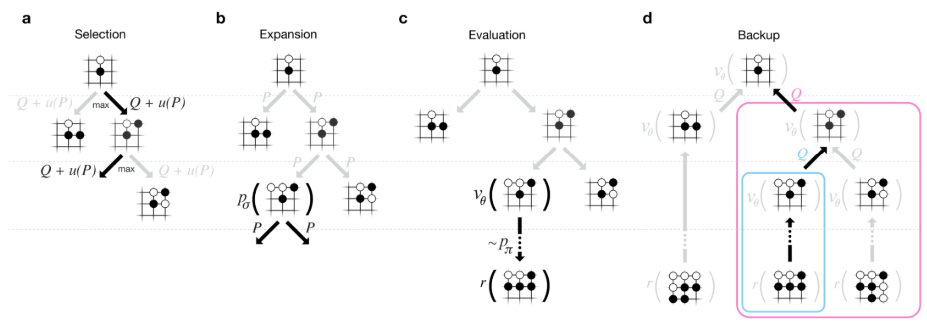
\includegraphics[width=0.8\textwidth]{Bilder/monte-carlo.png}
    \caption{AlphaGo Monte-Carlo tree search. Image from \autocite{alphago}}
    \label{fig:monecarlo}
\end{figure}

The internal model can also be learned by the \ac{RL} algorithm. \textcite{alphagoimprovementmuzero} modified the algorithm of \textcite{alphago} to learn the internal model. The modified algorithm was applied to different kinds of problems, including single player continuous state and action spaces. 


%Another major improvement in the domain of \ac{RL} was the combination of \acp{NN} with traditional planning and search algorithms, the most famous example for this is AlphaGo \textcite{alphago}. These algorithms often are model-based algorithms and use search algorithms (e.g. Monte Carlo Tree Search)  to evaluate the possible actions at a given state. The \acp{NN} are used for the evaluation of states and actions in the search algorithms. AlphaGo was developed for a 2 player deterministic game with a discrete state and action space. Since then this combination of \acp{NN} and search algorithms has also been used to achieve impressive results for all kinds of problems \textcite{alphafold}, for example single player continuous state and action spaces \textcite{alphagoimprovementmuzero}. Although these algorithms could be applied to the problem at hand, they will not be utilized due to the increased complexity of the algorithms and the required computational resources.


\subsubsection{Comparison of Model-Free and Model-Based Algorithms}

State of the art model-free and model-based algorithms have been used to solve all kind of \ac{RL} tasks. Both approaches can be applied to the task of autonomous driving. The model-free \ac{PPO} algorithm is used to train the agents in this thesis for a number of reasons. Model-free approaches are generally much simpler to implement since they do not require an internal model. Model-free algorithms also require less resources for the training and evaluation process.

%  find a citation for this



\subsection{\acp{CNN} for \ac{RL}}

\acp{CNN} are a \ac{NN} architecture specifically developed for processing image data, they consist of a number of filters and a fully connected \ac{NN}. The filters are applied to the image in a sliding window fashion. The filters detect patterns in the image such as edges and corners. Multiple successive applications of such filters enable the network to learn hierarchical information and recognize more complex structures. The fully connected \ac{NN} analyses the results of the filters and makes the final prediction \textcite{rlbook2020}.

\acp{CNN} are often used in \ac{RL} since RL problems often require an agent to process visual input. Compared to other feature extraction methods, \acp{CNN} can be trained end-to-end using the loss functions defined by the \ac{RL} algorithms. \acp{CNN} can learn what features are important for the task at hand.
Therefore a \ac{CNN} will be used to process the camera images instead of a hand-crafted feature extraction method. 

\acp{CNN} can take the raw camera/simulation images as input. Preprocessing steps are often applied to these images, e.g. grayscaling by \textcite{atari}. 



\subsubsection{Preprocessing Steps for \acp{CNN}}

There are many reasons for applying preprocessing steps to images for the use by \acp{CNN}. The images can be preprocessed to make the processing less computationally demanding, both in terms of processing speed and memory requirements. Preprocessing steps can also be applied with the goal of improving the performance of the \ac{NN} during training and evaluation. 

Preprocessing steps can change the image's height, width and channel dimensions. The datatype of an image can also be changed. The image's pixel values can also be changed.

The most common preprocessing step is grayscaling, the image's RGB color values are converted to a single grayscale value. This reduces the image's channel dimension from 3 to 1. Grayscaling reduces the computational requirements in terms of processing and memory. Furthermore it can improve the performance of the \ac{CNN}. Grayscaling can also improve the network's generalization to different environments. The network does not have to learn to recognize objects based on their color. The grayscaling step removes color information from the image. This can be a disadvantage if the color information is important for the task at hand.
\textcite{atari} used the grayscaling preprocessing step to make the processing less computationally demanding. 


The image's width and height dimensions can be changed with different preprocessing steps. Images can be cropped to a smaller size. Cropping can also remove irrelevant parts of the image or change the aspect ratio of the image. \textcite{atari} used cropping to achieve square images for GPU processing. Images can also be resized without significantly changing the image's semantic content using upsampling or downsampling. Similar to grayscaling the reduction of the image size results in less memory and processing requirements.

Normalization is another common preprocessing step. The pixel values of the image are rescaled. The rescaling can be done by multiplication with a factor, for example from the range $[0,255]$ to the ranges $[0,1]$ or $[-1, -1]$. Another common normalization approach standardizes the pixels to have a mean of 0 and a standard deviation of 1. Normalization approaches can improve the performance of the \ac{CNN} during training, \autocite{cnn_norm}.

Data augmentation can be applied to images during the training phase of the \ac{CNN}. This can help in improving the generalization of the CNN by making it robust to variations in the input data, \autocite{cnn_data_augmentation}.

Preprocessing steps that increase the contrast of images can increase the performance of \ac{CNN} algorithms. The increased contrast can make the image features more distinguishable. This can increase the \ac{CNN} performance. \textcite{cnn_contrast} review different approaches to increasing the image contrast, they show that contrast increasing steps can improve the performace of \acp{CNN}.

% rlbook2020 chapter 9.7 explains the use of \acp{CNN} in RL


\subsection{Extensions to \ac{RL}}

\subsubsection{Reward Shaping}
Reward shaping involves modifying the reward signal to guide the learning process more effectively. The term shaping comes from psychology and describes the idea of rewarding all behaviour that leads to the desired behaviour \autocite{rlbook2020}.

Reward signals are often sparse in \ac{RL} tasks. Sparse reward signals assign non-zero rewards only in a few steps and can make learning difficult. This makes it difficult for the agent to learn which actions lead to future rewards.

Reward shaping allows for the creation of a shaped reward function that gives frequent rewards for actions that lead to the desired behaviour. The agent can learn desired behaviours faster and more efficiently. 

Reward shaping can lead to unintended behaviour if the shaped reward function is not aligned with intended reward function. The agent can learn to exploit the shaped reward function and not learn the desired behaviour, \textcite{drl_for_ad}. 
To avoid this problem, the shaped reward function can be changed over time to the intended reward function, \textcite{rlbook2020}.


%drl paper reward shaping

\subsubsection{Memory Mechanisms}
\ac{RL} algorithms are often employed in dynamic environments, such as self-driving. The agent has to remember past experiences to have an accurate representation of the current dynamic environment state. Various memory mechanisms can be used by the agent to make decisions. 

Memory mechanisms typically store a fixed or variable amount of past observations. The stored observations are used together with the current observation to make decisions.

All \ac{NN} architectures are able to process sequences of fixed length. The sequence of stored and current observations is concatenated to produce a fixed size input for the \ac{NN}. This was used in the \ac{DQN} algorithm by \textcite{atari}. This implementation of the memory mechanism was also used by \textcite{maximilian} to build an agent that can traverse the tracks in the arena.


\acp{RNN} can be used to process sequences with varying length. The sequence of stored and current observations are fed into the \ac{RNN} to produce a representation of the environment state that includes past observations. \acp{LSTM} are a special version of \acp{RNN}. \textcite{lstm_ramp} used an \ac{LSTM} agent act in a dynamic ramp merging scenario.


\subsubsection{Domain Adaptation}

\acp{NN} are often trained in a simulated environment and then transferred to the real world. The \acs{NN} often perform poorly in the real world due to differences between the environments. This difference is called the \ac{S2R} gap. The \ac{S2R} gap has been studied extensively by researchers in the field of computer vision \autocite{sim2RealGap_rl} and \ac{RL} \autocite{sim2RealGap_vision}. The \ac{S2R} gap can be reduced by using domain adaptation techniques.

The \ac{S2R} gap can be reduced matching the simulated environment closely to reality. This can be done using high quality RGB renderings of the real-world environment for image processing agents. A more successful approach was the inclusion of additional depth sensors in the simulated environment. 

Trained models can be fine-tuned to the real world environment. The model is trained in simulation. The trained model is fine-tuned with a dataset of real-world data. \textcite{sim2RealGap_rl} used this approach to train a robotic agent in simulation using \ac{RL} and then fine-tuned it in the real world. 

Another domain adaptation approach tries to reduce the \ac{S2R} gap by training the agent on a diverse set of environment variations. The agent is trained in a wide range of environments that are generated by randomizing the environment's parameters. For example the object textures and the agent motor power. The agent learns to generalize to the environment variations. The agent is transferred to the real world without fine-tuning. In the best case, the real-world appears to the model as just another variation. \textcite{sim2RealGap_vision} used this approach to train a robotic object focusing agent in simulation.


\section{\acl{IL} for Self-Driving}
As described before it is difficult to build self-driving agents for real world environments due to the environment complexity. The amount of complex edge cases make it very difficult to programmatically define the agent's behaviour. \ac{ML} algorithms such as \ac{RL} can be used to control the agent behaviour instead. 
\ac{IL} is another approach to training an agent that interacts with its environment. \ac{IL} requires a dataset that demonstrates the desired behaviour. The agent is trained on the dataset to mimic the expert behaviour.

In \ac{RL} the programmer has to define a reward function that the agent uses to learn and improve its behaviour. In \ac{IL} the agent learns exclusively from the dataset. As a result this dataset has to include a wide range of scenarios to produce a reliable agent that can handle edge cases.

There are two common approaches to training an agent with \ac{IL}, \ac{BC} and \ac{IRL}. \ac{BC} is the simpler approach. The agent learns to mimic the expert behaviour directly. This is similar to supervised learning. \ac{IRL} is more complex. The reward function is learned from the expert demonstrations first. The agent is then trained to maximize this reward function using \ac{RL}.

Bojarski \textcite{bojarski2016endToEnd} used \ac{IL} to train a self-driving lane following agent for real-world environments. This agent consists of a \ac{CNN} that processes the camera images and predicts the steering angle directly. This \ac{NN} is trained end-to-end to reproduce steering behaviour from recorded data. They demonstrate that \ac{IL} is a viable approach for developing an autonomous driving steering agent without the need for multiple components such as object detection and path planning.

Tesla used \ac{IL} to train the path prediction component of their self-driving systems. The fleet of Tesla vehicles allows them to collect a large amount of representative data in the real world. The reference dataset was generated from recordings of human Tesla drivers \textcite{tesla_youtube}. 

\ac{IL} and \ac{RL} can be combined to improve the training of the agent. The \ac{RL} process generates samples via interaction between agent and environment. These samples and the expert behaviour dataset are used together to train the agent policy. \textcite{car-following_carla_dresden} used this approach to train a car following agent.



\section{Simulation for \ac{RL} and Self-Driving}

Simulations play a huge role in \ac{RL} and the development of self-driving agents. Simulations provide a huge number of benefits over real world experiments. They are much cheaper and faster to run than real world experiments. Furthermore they can be run in parallel. In addition the programmers have direct and perfect control over the environment, as such programmers can for example change the simulation speed. This allows for fast experimentation and training of \ac{RL} agents. Simulations also allow for the creation of scenarios that are not feasible in the real world. This is especially useful for \ac{RL} agents that are trained to avoid collisions. Simulations also allow for the creation of ground truths such as perfect sensor data and object bounding boxes.

Interest in self-driving has also led to the development of dedicated simulators, such as the Carla by \textcite{carla} and the AirSim by \textcite{airsim} simulator. The Carla simulator provides researchers with useful features such as weather control and ground truths for object detection and segmentation.

Simulated environments often serve as baselines for \ac{RL} algorithms, most famous are the atari games by \textcite{atari}. \textcite{gymnasium} developed the Python Gymnasium API for easy reuse and comparison of \ac{RL} algorithms for different problems. The Gymnasium API defines an interface that can be used to model tasks as \ac{RL} problems. A wide range of \ac{RL} frameworks support the Gymnasium API, for example Google's dopamine by \textcite{dopamine} and OpenAI's \ac{SB3} by \textcite{sb3}. 

Advanced simulations like the Unity engine \autocite{unity} and the physics simulator MuJoCo \autocite{mujoco} can be integrated with the Gymnasium API.
Some dedicated \ac{RL} frameworks integrate directly with simulation engines. \textcite{maximilian} used the ML-Agents framework \textcite{mlagents} to train the self-driving agent in Unity directly.

Unity will be used for the simulation in this thesis, the simulation will be integrated with the Python Gymnasium API and \ac{PPO} algorithm. Compared to the ML-Agents framework, this allows for more flexibility and control over the simulation and training process.

